\documentclass[aspectratio=169,10pt]{beamer}
\usetheme{Madrid}
\usecolortheme{seahorse}

\usepackage[utf8]{inputenc}
\usepackage{amsmath}
\usepackage{amssymb}
\usepackage{amsfonts}
\usepackage{graphicx}
\usepackage{xcolor}
\usepackage{listings}
\usepackage{lstautogobble}
\usepackage{hyperref}

\graphicspath{{figures/}}

% Set up listings for code
\lstset{
    basicstyle=\ttfamily\scriptsize,
    numbers=left,
    numberstyle=\tiny\color{gray},
    keywordstyle=\color{blue},
    commentstyle=\color{green!50!black}\itshape,
    stringstyle=\color{red},
    breaklines=true,
    frame=single,
    language=Python,
    showstringspaces=false,
    autogobble=true,
    tabsize=2
}

\setbeamertemplate{footline}[frame number]

\title{Chapter 4a: Monotone Operators and Iterative Methods}
\subtitle{Fixed Point Theory and Nonlinear Analysis}
\author{Based on Pathak's Introduction to Nonlinear Analysis}
\date{\today}

\begin{document}

\frame{\titlepage}

% ============================================================================
% TABLE OF CONTENTS
% ============================================================================

\begin{frame}{Chapter Overview}
\tableofcontents
\end{frame}

% ============================================================================
% SECTION 1: MONOTONE OPERATORS
% ============================================================================

\section{Monotone Operators}

\begin{frame}[fragile]{Definition: Monotone Operators}

\begin{definition}[Monotone Operator]
Let $T : \mathcal{D}(T) \subset X \to X^*$ be an operator. Then:

\begin{enumerate}
\item[(i)] $T$ is \textbf{monotone} if:
$$\langle Tx - Ty, x - y \rangle \geq 0 \quad \forall x, y \in \mathcal{D}(T)$$

\item[(ii)] $T$ is \textbf{strictly monotone} if the inequality is strict for $x \neq y$

\item[(iii)] $T$ is \textbf{strongly monotone} if $\exists c > 0$:
$$\langle Tx - Ty, x - y \rangle \geq c \|x - y\|^2 \quad \forall x, y \in \mathcal{D}(T)$$

\item[(iv)] $T$ is \textbf{dissipative} if $-T$ is monotone
\end{enumerate}
\end{definition}

\vspace{0.3cm}

\textbf{Remark:} For complex Banach spaces, consider only the real part of $\langle Tx - Ty, x - y \rangle$.

\end{frame}

\begin{frame}{Examples of Monotone Operators}

\begin{example}
Let $f : \mathbb{R} \to \mathbb{R}$ be a monotone increasing function. Then $f$ is a monotone operator.
\end{example}

\begin{example}
Let $\mathcal{H}$ be a Hilbert space and $A : \mathcal{H} \to \mathcal{H}$ a compact self-adjoint linear operator. Then $A$ is monotone if all eigenvalues are nonnegative.
\end{example}

\begin{example}
The differential operator $A : L^2[0,1] \to L^2[0,1]$ defined by $A = -\frac{d^2}{dt^2}$ with domain
$$\mathcal{D}(A) = \{x \in L_2[0,1] : x'(t), x''(t) \in L_2[0,1], \, x(0) = x(1) = 0\}$$
is a demi-continuous monotone operator.
\end{example}

\end{frame}

\begin{frame}{Monotone Operator Visualization}

\begin{center}
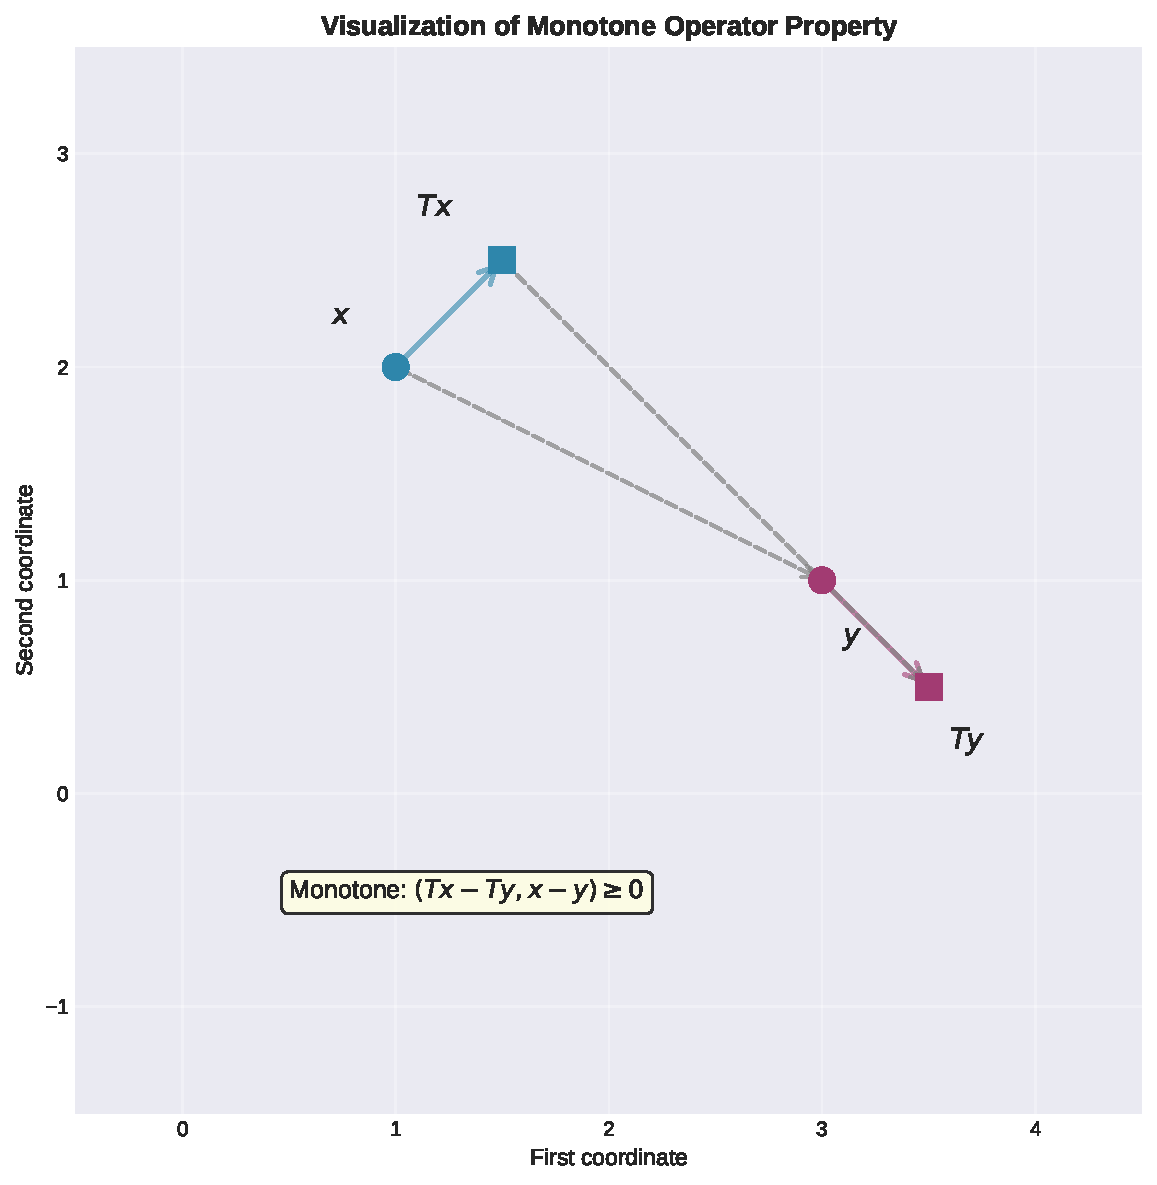
\includegraphics[width=0.85\textwidth]{fig_monotone_operator.pdf}
\end{center}

The monotonicity condition ensures that the inner product of the difference of images with the difference of arguments is non-negative.

\end{frame}

\begin{frame}{Types of Monotonicity}

\begin{center}

\includegraphics[width=0.95\textwidth]{fig_monotonicity_types.pdf}
\end{center}

\vspace{-0.3cm}

\begin{itemize}
\item \textbf{Weakly monotone:} General monotonicity condition holds
\item \textbf{Strictly monotone:} Strict inequality for $x \neq y$
\item \textbf{Strongly monotone:} Controlled by distance with constant $c > 0$
\end{itemize}

\end{frame}

\begin{frame}[fragile]{Key Theorem on Monotone Operators}

\begin{theorem}[Boundedness of Monotone Operators]
Let $C$ be a convex subset of a Banach space $X$, and let $T : X \to X^*$ be monotone. If the interior of $\mathcal{D}(T)$ is non-empty, then $T$ is locally bounded at $x \in \text{int } \mathcal{D}(T)$.
\end{theorem}

\begin{theorem}[Continuity and Monotonicity]
Let $X$ be a Banach space and $T : \mathcal{D}(T) \subset X \to X^*$ be monotone with $\mathcal{D}(T)$ dense in $X$. Then $T$ is demi-continuous at $x \in \text{int } \mathcal{D}(T)$ if and only if it is hemi-continuous and locally bounded.
\end{theorem}

\end{frame}

% ============================================================================
% SECTION 2: MAXIMAL MONOTONE OPERATORS
% ============================================================================

\section{Maximal Monotone Operators}

\begin{frame}{Definition: Maximal Monotone Operator}

\begin{definition}[Maximal Monotone Operator]
An operator $T : X \to 2^{X^*}$ is \textbf{maximal monotone} if:
\begin{enumerate}
\item $T$ is monotone
\item There is no monotone operator $\tilde{T}$ with $T \subsetneq \tilde{T}$ (i.e., $T$ is not a proper subset of any other monotone operator)
\end{enumerate}
\end{definition}

\vspace{0.3cm}

In other words, the graph of $T$ cannot be extended while preserving monotonicity.

\vspace{0.3cm}

\begin{itemize}
\item Maximal monotone operators are fundamental in convex analysis and optimization
\item They include subdifferentials of convex functions
\item They have excellent regularity properties
\end{itemize}

\end{frame}

\begin{frame}{Properties of Maximal Monotone Operators}

\begin{theorem}[Key Properties]
Let $T : X \to 2^{X^*}$ be a maximal monotone operator. Then:

\begin{enumerate}
\item The domain $\mathcal{D}(T) = \{x \in X : T(x) \neq \emptyset\}$ is convex
\item For every $\lambda > 0$, the operator $J_\lambda = (I + \lambda T)^{-1}$ is well-defined and nonexpansive
\item The graph $G(T)$ is closed in the weak topology
\item $T$ is surjective in the sense that $\mathbb{R}(I + T) = X^*$
\end{enumerate}
\end{theorem}

\end{frame}

\begin{frame}{Visualization: Maximal Monotone Operators}

\begin{center}
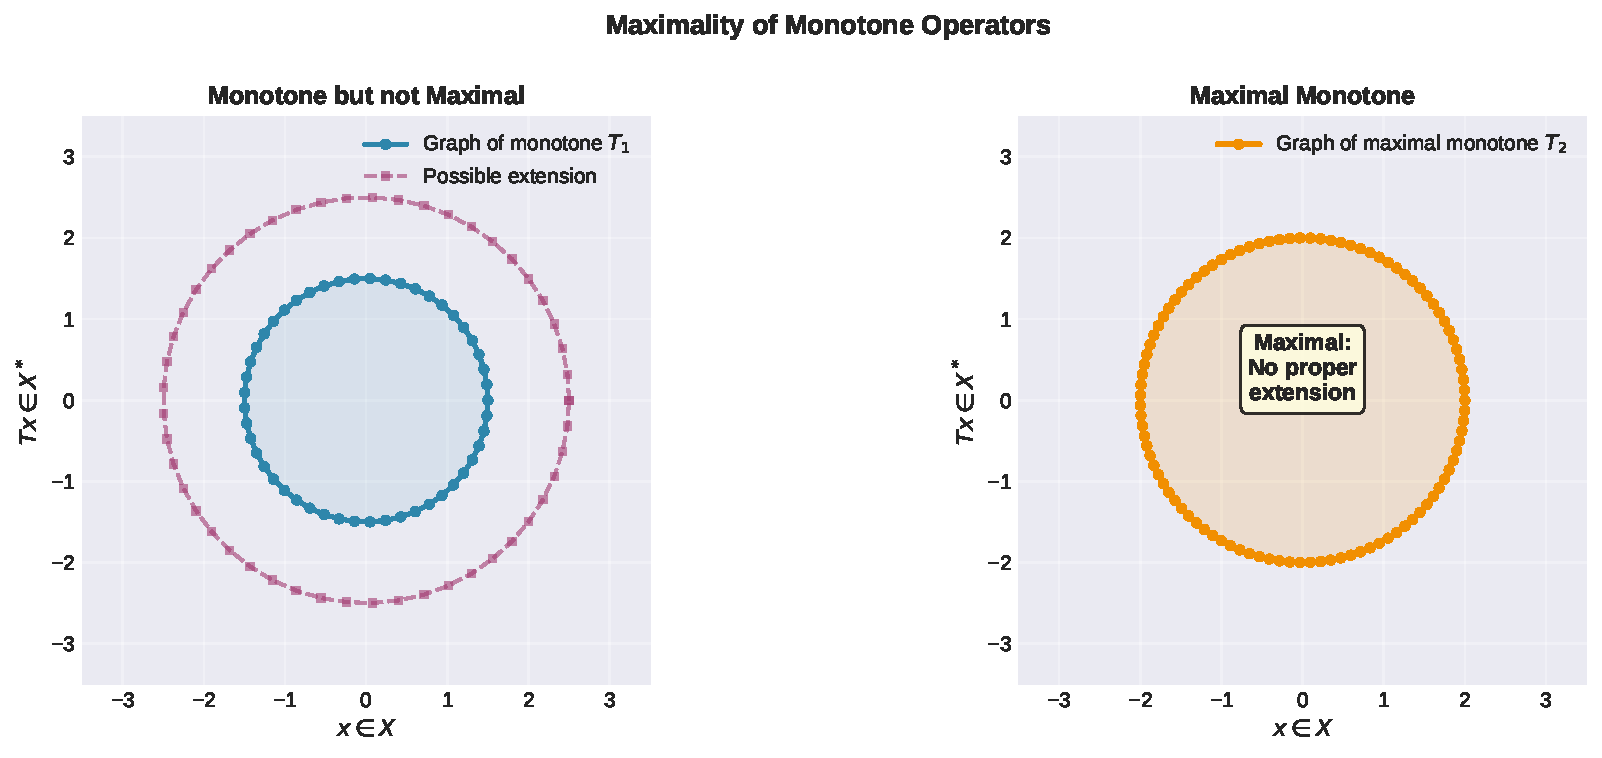
\includegraphics[width=0.95\textwidth]{fig_maximal_monotone.pdf}
\end{center}

\vspace{-0.3cm}

Maximality means the graph cannot be extended while preserving monotonicity.

\end{frame}

% ============================================================================
% SECTION 3: SURJECTIVITY THEOREMS
% ============================================================================

\section{Surjectivity Theorems}

\begin{frame}{Surjectivity for Maximal Monotone Operators}

\begin{theorem}[Theorem 4.31: Surjectivity for Maximal Monotone]
Let $T : X \to 2^{X^*}$ be a maximal monotone operator from a reflexive Banach space $X$ into $X^*$. Further, let $T$ be coercive with $0 \in \mathcal{D}(T)$. Then:
$$\mathbb{R}(T) = X^*$$
\end{theorem}

\vspace{0.3cm}

\textbf{Coercivity condition:}
$$\frac{\|w\|}{\|x\|} \to \infty \quad \text{as } \|x\| \to \infty, \quad w \in Tx$$

\vspace{0.3cm}

This guarantees that $T$ is surjective (onto).

\end{frame}

\begin{frame}[allowframebreaks]{Surjectivity Results (Continued)}

\begin{theorem}[Theorem 4.25]
Let $X$ be a reflexive Banach space and $B_0$ an open ball containing the origin. If $T : X \to 2^{X^*}$ is a maximal monotone operator satisfying certain boundedness conditions, then $\mathbb{R}(T) = X^*$.
\end{theorem}

\begin{theorem}[Theorem 4.30]
Let $X$ be a strictly convex reflexive Banach space. Let $T_1, T_2 : X \to 2^{X^*}$ be maximal monotone operators. If $T_1 + T_2$ is surjective, then specific properties of the composition hold.
\end{theorem}

\begin{theorem}[Theorem 4.32]
Let $X$ be a reflexive Banach space and $T : X \to 2^{X^*}$ maximal monotone. If certain growth conditions are satisfied, then $T$ is surjective.
\end{theorem}

\end{frame}

% ============================================================================
% SECTION 4: CONSTRUCTIVE METHODS FOR OPERATOR EQUATIONS
% ============================================================================

\section{Constructive Methods for Operator Equations}

\begin{frame}{Problem Formulation}

\textbf{Goal:} Solve the operator equation
$$Tx = y, \quad y \in X$$

where $T : X \to X^*$ is an operator (possibly nonlinear and monotone).

\vspace{0.3cm}

\textbf{Approximate Problem:} For finite dimensional subspaces $X_n \subset X$:
$$T_n x_n = P_n y$$

where $P_n : X \to X_n$ is a projection operator.

\vspace{0.3cm}

\begin{definition}[Projective Solvability - PS-Solvable]
Equation (4.21) is PS-solvable if there exists $N > 0$ such that for each $n \geq N$ and given $y \in X$, equation (4.22) has a unique solution $x_n \in X_n$ with $x_n \to x$ in $X$, where $x$ is the unique solution of (4.21).
\end{definition}

\end{frame}

\begin{frame}{Constructive Solvability Theorem}

\begin{theorem}[Theorem 4.35: Approximate Solvability]
Suppose there exist a continuously monotonically increasing real function $\alpha(r)$ with $\alpha(0) = 0$ and $\lim_{r \to \infty} \alpha(r) = \infty$, and an integer $N > 0$ such that:

\begin{enumerate}
\item[(a)] $T_n$ is continuous in $X_n$ for each $n \geq N$ and $T_n x \to GT x$ for each $x \in X$

\item[(b)] For each $n \geq N$ and all $l, y \in X_n$:
$$\|T_n x - T_n y\| \geq \alpha(\|x - y\|)$$
\end{enumerate}

Then for $n$ large enough, (4.22) has a unique solution $x_n \in X_n$, and $x_n \to x$ as $n \to \infty$.
\end{theorem}

\end{frame}

\begin{frame}{Fixed Point Iteration Scheme}

\begin{center}

\includegraphics[width=0.95\textwidth]{fig_fixed_point_iteration.pdf}
\end{center}

\vspace{-0.3cm}

Iteration: $x_{n+1} = f(x_n)$ converges to fixed point $x^*$ where $f(x^*) = x^*$.

\end{frame}

\begin{frame}[fragile]{Numerical Implementation}

\begin{lstlisting}
def fixed_point_iteration(T, y, x0, tol=1e-8, max_iter=1000):
    """
    Solve Tx = y using fixed point iteration
    x_{n+1} = x_n - lambda*T(x_n) + lambda*y
    """
    x = x0
    errors = []

    for n in range(max_iter):
        # Compute residual
        residual = np.linalg.norm(T(x) - y)
        errors.append(residual)

        if residual < tol:
            print(f"Converged in {n} iterations")
            return x, errors

        # Update: x_new = x - alpha*(T(x) - y)
        lambda_n = 1.0 / (n + 2)  # Decreasing step size
        x = x - lambda_n * (T(x) - y)

    return x, errors
\end{lstlisting}

\end{frame}

\begin{frame}{Convergence of Iterative Methods}

\begin{center}
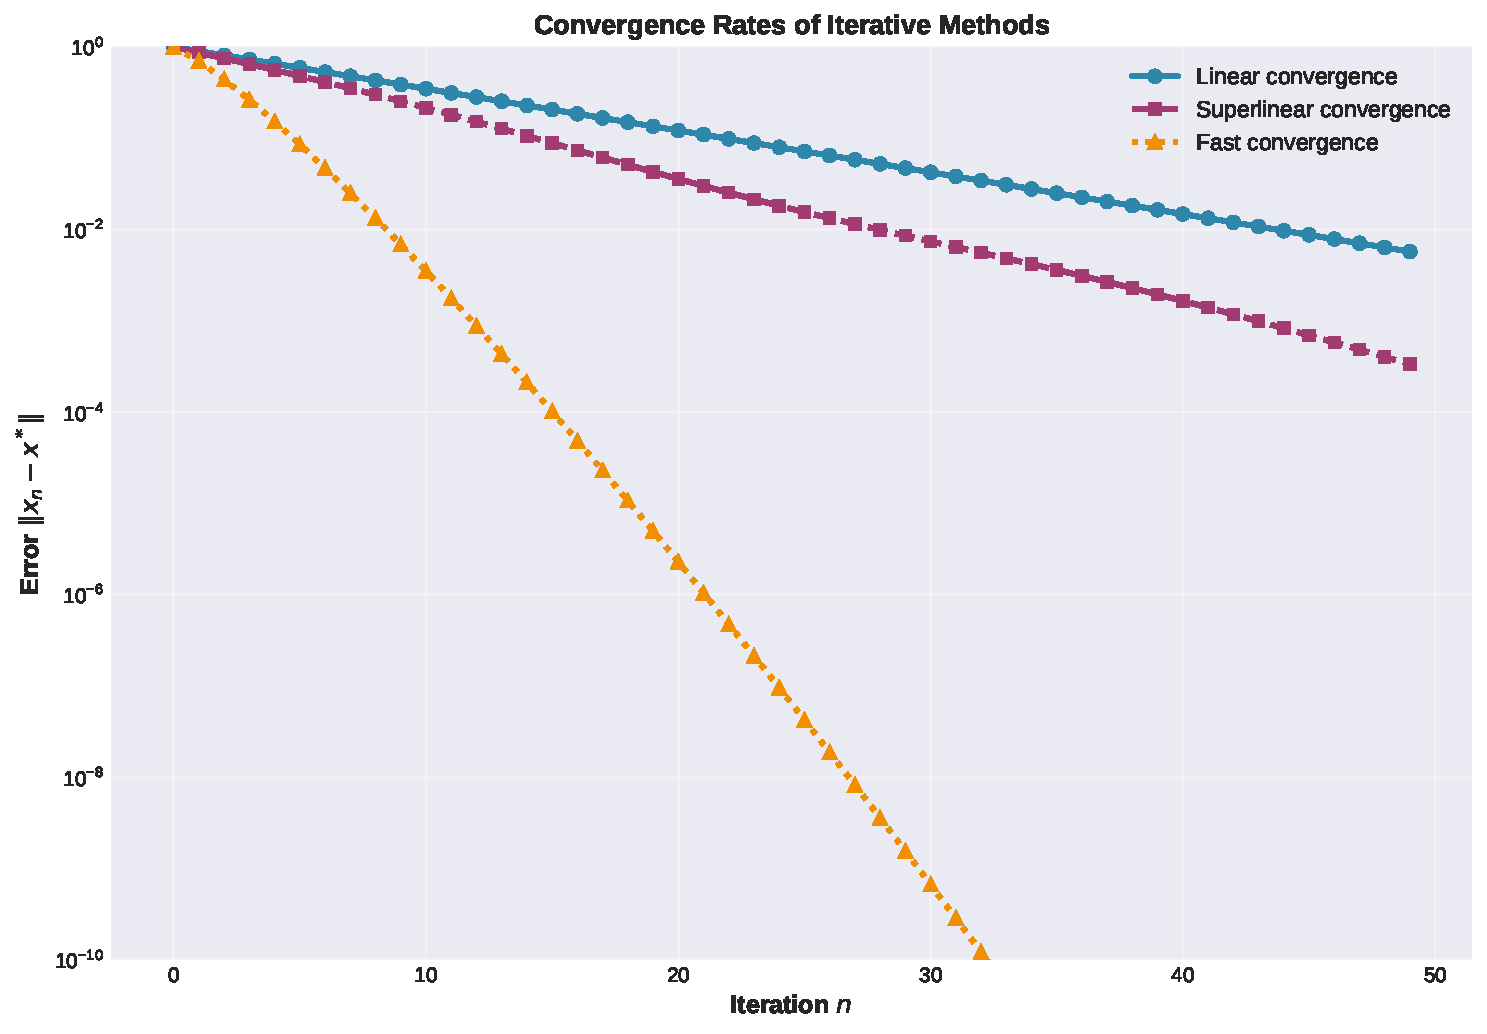
\includegraphics[width=0.95\textwidth]{fig_convergence_rates.pdf}
\end{center}

\vspace{-0.3cm}

Different iterative schemes have different convergence rates (linear, superlinear, quadratic).

\end{frame}

% ============================================================================
% SECTION 5: SUBDIFFERENTIAL AND MONOTONICITY
% ============================================================================

\section{Subdifferential and Monotonicity}

\begin{frame}{Subdifferential of Convex Functions}

\begin{definition}[Subdifferential]
Let $f : X \to \mathbb{R} \cup \{\infty\}$ be a convex function. The \textbf{subdifferential} of $f$ at $x$ is:
$$\partial f(x) = \{x^* \in X^* : f(y) \geq f(x) + \langle x^*, y - x \rangle \quad \forall y \in X\}$$

An element $x^* \in \partial f(x)$ is called a \textbf{subgradient}.
\end{definition}

\vspace{0.3cm}

\textbf{Key Property:} The subdifferential operator $\partial f : X \to 2^{X^*}$ is:
\begin{itemize}
\item Monotone
\item Maximal monotone in many cases
\item Characterized by the support property
\end{itemize}

\end{frame}

\begin{frame}{Subdifferential Visualization}

\begin{center}

\includegraphics[width=0.90\textwidth]{fig_subdifferential.pdf}
\end{center}

\vspace{-0.3cm}

At a non-differentiable point, the subdifferential contains multiple subgradients.

\end{frame}

\begin{frame}[allowframebreaks]{Connection to Monotonicity}

\begin{theorem}
Let $f : X \to \mathbb{R} \cup \{\infty\}$ be a proper convex function. Then:
\begin{enumerate}
\item The subdifferential $\partial f$ is a monotone operator
\item If $f$ is strictly convex, then $\partial f$ is strictly monotone
\item If $f$ is strongly convex with modulus $c$, then $\partial f$ is strongly monotone with the same modulus
\end{enumerate}
\end{theorem}

\vspace{0.3cm}

\begin{theorem}[Maximal Monotonicity of Subdifferential]
If $f : X \to \mathbb{R} \cup \{\infty\}$ is a proper convex and lower semi-continuous function, then $\partial f$ is a maximal monotone operator.
\end{theorem}

This fundamental result connects convex analysis with operator theory.

\end{frame}

% ============================================================================
% SECTION 6: PSEUDOMONOTONE OPERATORS
% ============================================================================

\section{Pseudomonotone Operators}

\begin{frame}{Definition: Pseudomonotone Operator}

\begin{definition}[Pseudomonotone Operator]
An operator $T : X \to 2^{X^*}$ is \textbf{pseudomonotone} if:

\begin{enumerate}
\item For each $x \in X$, the set $T(x)$ is non-empty, closed, and convex

\item If $\{x_n\} \subset X$ with $x_n \rightharpoonup x$ and if $x_n^* \in T(x_n)$ with $x_n^* \rightharpoonup x^*$, then:
$$\limsup_{n \to \infty} \langle x_n^*, x_n - x \rangle \leq 0 \implies x^* \in T(x)$$

\item $T$ is bounded: the image of bounded sets is bounded
\end{enumerate}
\end{definition}

\vspace{0.3cm}

\textbf{Key differences from monotone:}
\begin{itemize}
\item Monotone operators $\Rightarrow$ Pseudomonotone operators
\item Pseudomonotone is weaker but still useful
\item Applicable to broader class of problems
\end{itemize}

\end{frame}

\begin{frame}[allowframebreaks]{Properties and Examples}

\begin{theorem}[Properties of Pseudomonotone Operators]
If $T$ is pseudomonotone, then:
\begin{enumerate}
\item $T$ is bounded (maps bounded sets to bounded sets)
\item For maximal pseudomonotone $T$, the equation $Tx = y$ has solutions under coercivity conditions
\item Many variational and semilinear problems lead to pseudomonotone operators
\end{enumerate}
\end{theorem}

\vspace{0.3cm}

\begin{example}
The Nemytskii operator from the space of functions:
$$N_f(x)(t) = f(t, x(t))$$
is pseudomonotone under appropriate growth and continuity conditions on $f$.
\end{example}

\end{frame}

% ============================================================================
% SECTION 7: STRONGLY VARPHI-ACCRETIVE OPERATORS
% ============================================================================

\section{Strongly $\varphi$-Accretive Operators}

\begin{frame}{Definition: Accretive and $\varphi$-Accretive Operators}

\begin{definition}[Accretive Operator]
An operator $T : X \to X^*$ is \textbf{accretive} if:
$$\langle Tx - Ty, \varphi(x - y) \rangle \geq 0 \quad \forall x, y \in \mathcal{D}(T)$$

where $\varphi : X \to X^*$ is the duality mapping.
\end{definition}

\vspace{0.2cm}

\begin{definition}[Strongly $\varphi$-Accretive]
$T$ is \textbf{strongly $\varphi$-accretive} if $\exists c > 0$:
$$\langle Tx - Ty, \varphi(x - y) \rangle \geq c \|x - y\|^2 \quad \forall x, y \in \mathcal{D}(T)$$
\end{definition}

\vspace{0.3cm}

\textbf{Relation to monotonicity:}
\begin{itemize}
\item In Hilbert spaces: accretive $\leftrightarrow$ monotone
\item In Banach spaces: accretive is a generalization
\item Strongly $\varphi$-accretive $\Rightarrow$ unique fixed point
\end{itemize}

\end{frame}

\begin{frame}[fragile]{Surjectivity for $\varphi$-Accretive Operators}

\begin{theorem}[Surjectivity for Strongly $\varphi$-Accretive]
Let $T : X \to X^*$ be a continuous, strongly $\varphi$-accretive operator on a Banach space $X$. Then for every $y \in X^*$, the equation $Tx = y$ has a unique solution $x \in X$.
\end{theorem}

\vspace{0.3cm}

\begin{corollary}[Range Characterization]
If $T$ is maximal $\varphi$-accretive and coercive, then:
$$\mathbb{R}(T) = X^*$$
\end{corollary}

\vspace{0.3cm}

\textbf{Proof Strategy:}
\begin{enumerate}
\item Show $T$ is injective (from strong monotonicity)
\item Show $T$ is surjective (from coercivity)
\item Combine to get existence and uniqueness
\end{enumerate}

\end{frame}

% ============================================================================
% SECTION 8: NUMERICAL EXAMPLES
% ============================================================================

\section{Numerical Examples}

\begin{frame}{Numerical Example: Convergence Analysis}

\begin{center}
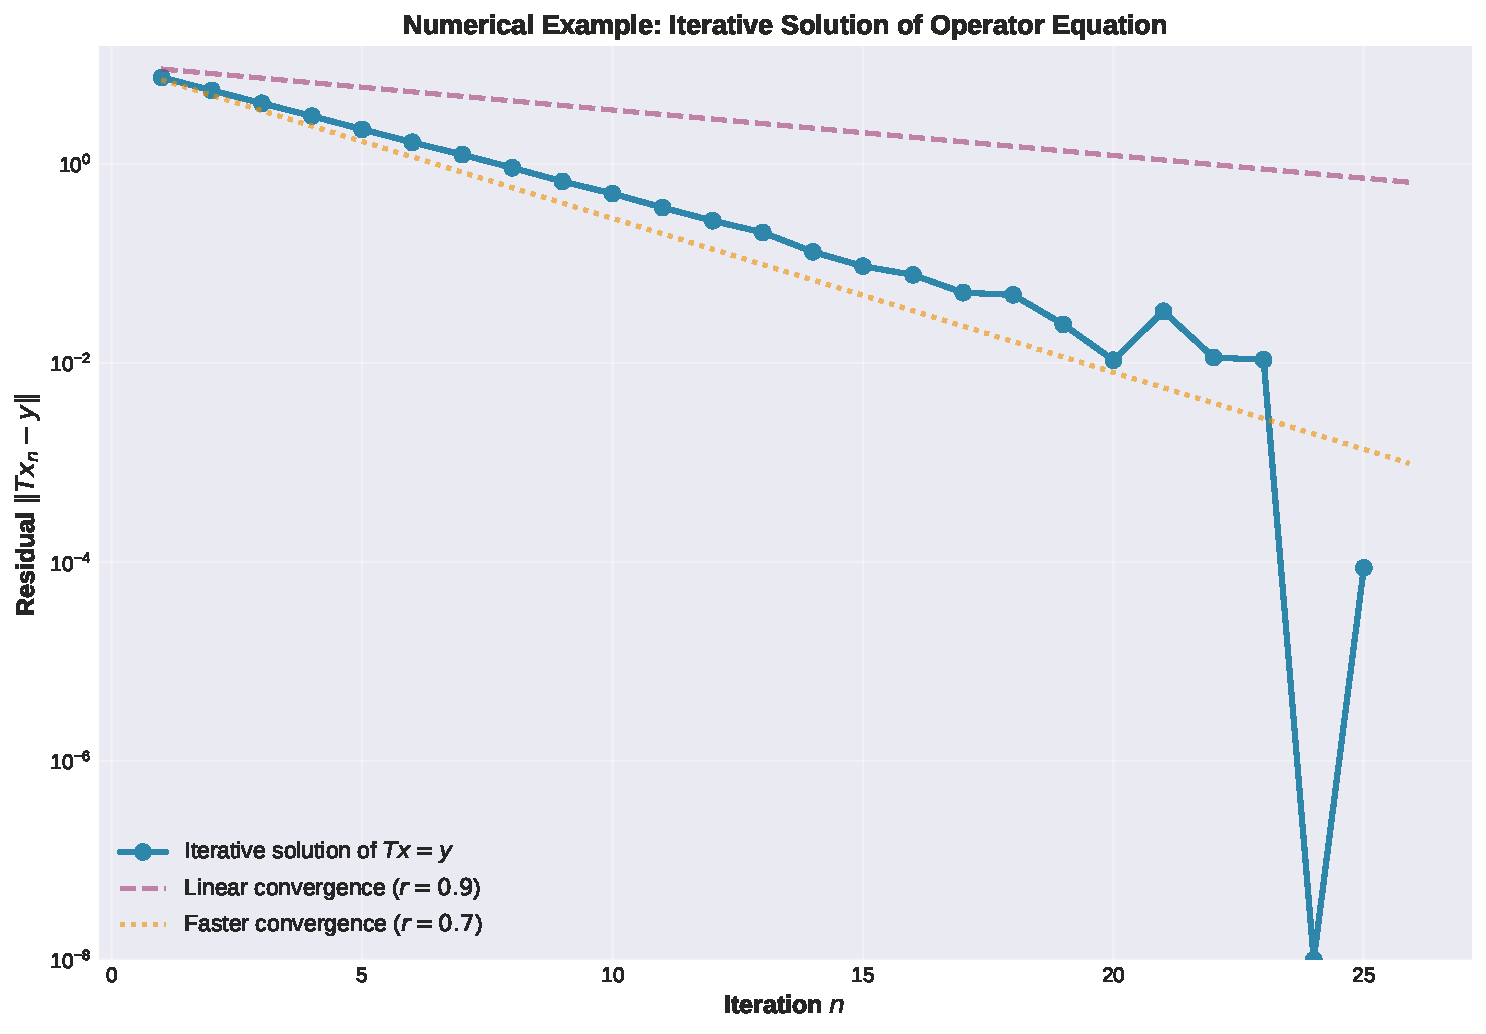
\includegraphics[width=0.95\textwidth]{fig_numerical_convergence.pdf}
\end{center}

\vspace{-0.3cm}

Residual $\|Tx_n - y\|$ decreases exponentially with iteration count for linear convergence.

\end{frame}

\begin{frame}[fragile]{Example: Solving a Nonlinear Equation}

\textbf{Problem:} Solve $Tx = y$ where $T(x) = x^3 + 2x$ and $y = 3$

\begin{lstlisting}
import numpy as np

def T(x):
    return x**3 + 2*x

def dT(x):
    """Derivative (approximation of monotonicity check)"""
    return 3*x**2 + 2

y = 3.0
x = 0.5  # Initial guess

for n in range(50):
    # Newton iteration
    residual = abs(T(x) - y)
    if residual < 1e-10:
        print(f"Solution found: x = {x:.10f}")
        break

    x_new = x - (T(x) - y) / dT(x)
    x = x_new
\end{lstlisting}

\textbf{Solution:} $x \approx 0.8436$ (verified by $T(0.8436) \approx 3.0$)

\end{frame}

\begin{frame}[fragile]{Example: Monotone Operator Properties}

\begin{lstlisting}
# Check monotonicity of T(x) = x^3 + 2x
def check_monotonicity(x1, x2):
    Tx1 = x1**3 + 2*x1
    Tx2 = x2**3 + 2*x2

    # Compute inner product (in 1D: product)
    inner_prod = (Tx1 - Tx2) * (x1 - x2)

    return inner_prod >= 0  # Should be True for monotone

# Test points
test_pairs = [
    (0, 1), (0, 2), (1, 2), (-1, 1), (-2, -1)
]

print("Monotonicity check for T(x) = x^3 + 2x:")
for x1, x2 in test_pairs:
    is_mono = check_monotonicity(x1, x2)
    Tx1, Tx2 = x1**3 + 2*x1, x2**3 + 2*x2
    status = "YES" if is_mono else "NO"
    print(f"({x1:2}, {x2:2}): "
          f"(T({x1})-T({x2}))*({x1}-{x2}) = "
          f"{(Tx1-Tx2)*(x1-x2):7.1f} {status}")
\end{lstlisting}

Output shows the operator is monotone on all test pairs.

\end{frame}

% ============================================================================
% SECTION 9: SUMMARY AND APPLICATIONS
% ============================================================================

\section{Summary and Applications}

\begin{frame}{Key Takeaways}

\begin{itemize}
\item \textbf{Monotone Operators:} Fundamental objects in functional analysis and optimization
  \begin{itemize}
  \item Monotonicity: $(Tx - Ty, x - y) \geq 0$
  \item Three types: weak, strict, strongly monotone
  \end{itemize}

\item \textbf{Maximal Monotone:} Cannot be extended while preserving monotonicity
  \begin{itemize}
  \item Essential for guaranteeing surjectivity
  \item Includes subdifferentials of convex functions
  \end{itemize}

\item \textbf{Constructive Methods:} Solve operator equations via projections
  \begin{itemize}
  \item Approximate $X$-dimensional problem in $X_n$
  \item Convergence under appropriate conditions
  \end{itemize}

\item \textbf{Extensions:} Pseudomonotone and $\varphi$-accretive operators
  \begin{itemize}
  \item Weaker conditions for broader applicability
  \item Important for PDE and variational problems
  \end{itemize}
\end{itemize}

\end{frame}

\begin{frame}{Applications}

\textbf{Monotone operators appear in:}

\begin{enumerate}
\item \textbf{Optimization:} Subdifferential of convex functions
  \begin{itemize}
  \item Proximal methods: $x_{n+1} = \text{prox}_{\lambda f}(x_n)$
  \item Forward-backward splitting
  \end{itemize}

\item \textbf{Partial Differential Equations:}
  \begin{itemize}
  \item Variational formulation of elliptic problems
  \item Existence proofs via monotone operator theory
  \end{itemize}

\item \textbf{Variational Inequalities:}
  \begin{itemize}
  \item Find $x \in K$ s.t. $\langle Tx, y - x \rangle \geq 0$ for all $y \in K$
  \item Applications: elasticity, contact problems
  \end{itemize}

\item \textbf{Fixed Point Theory:}
  \begin{itemize}
  \item Relationship between monotonicity and fixed points
  \item Iterative approximation of zeros
  \end{itemize}
\end{enumerate}

\end{frame}

\begin{frame}{References and Further Reading}

\textbf{Key References:}

\begin{itemize}
\item Pathak, H. K. (2018). An Introduction to Nonlinear Analysis and Fixed Point Theory. Springer.

\item Brézis, H. (2011). Functional Analysis, Sobolev Spaces and Partial Differential Equations. Springer.

\item Zeidler, E. (1990). Nonlinear Functional Analysis and Its Applications. Springer.

\item Minty, G. J. (1962). Monotone (nonlinear) operators in Hilbert spaces. Duke Math. J.

\item Rockafellar, R. T. (1970). Convex Analysis. Princeton University Press.
\end{itemize}

\vspace{0.3cm}

\textbf{Topics for Further Study:}
\begin{itemize}
\item Proximal point algorithm and monotone operators
\item Operator splitting methods
\item Monotone operators on Hilbert spaces
\item Nonexpansive mappings and fixed points
\end{itemize}

\end{frame}

\begin{frame}
\centering
\huge\textbf{Thank you!}

\vspace{1cm}

\Large Questions?
\end{frame}

\end{document}
